\scanpage{334}

plus gén., si $A\supset J$ est un Anneau à pd, \unsure{on a|est-ce} $F(J)\unsure{\rightharpoondown|{-}}F(A)$ inj, donc $F(J)$ à p div dans $F(A)$ ?

\diagram{\begin{tikzcd}
F(J)\arrow[r,"\mathrm{deg}\ p"] & F(J) \\
J\arrow[r,"\uline{\gamma^p}",no head] & J
\end{tikzcd}}
\margin{oui, en \unsure{transf|transport}}

\deleted{\unsure{F|k}} $A$ - donne la relation
\deleted{$(x\unsure{+|\circ}y)$}
\[
x,y\in F(\unsure{J|\varphi})\quad\Longrightarrow\quad
\underset{\Vert}{(x+y)^{\unsure{(p)|p}}}=\sum_{i+j=p}x^{(i)}y^{(j)}\quad?
\]
\[x,y\in\qquad u\]

\diagram{\begin{tikzcd}
\dot{\mathscr P}\arrow[r,"\overline F",no head] & \mathscr P'
\end{tikzcd}}
commute aux produits\par
conserve degré et degrés partiels
\margin{bidegrés $1,1$}

\deleted{donc il}
\[
A,J\qquad J\unsure{\hookrightarrow|\longrightarrow} A
\]
$A$ \inserted{$k$-}\unsure{ab groupe|\deleted{ab groupe}|algèbre} ass comm avec $1$\par
$J$ anneau ass comm sans $1$\par
$A$ opère sur $J$, et $(\lambda xy=x(\lambda y)=\lambda\unsure{x|a}y$
\[
J\xrightarrow{i} A\qquad\text{hom de }A\text{-}\text{algèbre}
\]
\[
(i(xy)=i(x)i(y)\qquad i(\lambda x)=\lambda i(x))
\]
\margin{\diagram{\begin{tikzcd}
A\times A\arrow[r,harpoon'] & A \\
A\times J\arrow[r,no head] & J
\end{tikzcd}}}
\[
k\longrightarrow\operatorname{Hom}_{\mathscr P}(\underset{\unsure{J|\jmath}}{0},A)\qquad\text{hom d'anneaux}
\]
\deleted{\unsure{appl fonct}}
\figure{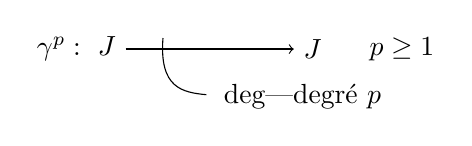
\begin{tikzpicture}
\node (source) at (0,0) {$\gamma^p:\ J$};
\node (target) at (3,0) {$J$};
\draw[->] (source.east)--(target.west);
\node[anchor=west] at (3.6,0) {$p\geq1$};
\draw (1.1,.14) .. controls (1.05,-.5) and (1.35,-.55) .. (1.65,-.58);
\node[anchor=west] at (1.75,-.6) {\unsure{deg|degré} $p$};
\end{tikzpicture}}
\margin{$\gamma^0:J-A$}
\[
\begin{aligned}
\gamma^0&=1\\
\gamma^1&=\mathrm{id}_J\\
\gamma^p(x+y)&=\sum_{i+j=p}\gamma^i x\,\gamma^j y\\
\gamma^p(\lambda a)&=\lambda^p\gamma^p(\unsure{a|u})\\
\gamma^p(\unsure{m|u})\gamma^q(\unsure{m|u})&=C_{pq}\gamma^{\unsure{p+q|pq}}(\unsure{m|u})\\
\gamma^p(\underset{:}{\gamma^q}(\unsure{m|u}))&=\frac{(pq)!}{(p!)^q q!}\gamma^{pq}(\unsure{m|u})
\end{aligned}
\]

\uline{\unsure{transfini|transformé} en \unsure{Ann|An}}
\diagram{\begin{tikzcd}
\Gamma^{\unsure{\alpha|k}}F(X)\arrow[r] & F\Gamma^\gamma(X)
\end{tikzcd}}

\mspage{335}
